% !TEX root = ../main.tex

\chapter{Experiments}
\label{ch:experiments}

\section{Research Questions}
To analyze and compare the different models, I formulated the following research questions:
\begin{enumerate}
  \item How do function approximators other than neural networks compare with the latter?
  \item Bias
\end{enumerate}

\section{Experiments}
To investigate and answer the formulated research questions, I conducted the following experiments:
\begin{enumerate}
  \item Similar to \citet{oller_analyzing_2020}, I used RWG to draw the weights of the models and tested the performance on a Classic Control environment from OpenAI Gym.
  \item Second experiment
\end{enumerate}
In the first experiment, analogous to \citet{oller_analyzing_2020}, there is no learning involved. For their paper, they were interested in the complexity of the environment, whereas I aim to find out more about the nature of the models. I selected a few candidates for the models, which are described in Section~\ref{ssec:models} and used them for a series of experiments. I used the same procedure for all models, which allows me to compare them with one another. For the experiments, first, I initialized the environment. I used the \verb|CartPole| and \verb|Acrobot| environment for these experiments. These environments are fairly easy to solve, as explained in Section~\ref{ssec:benchmarks}. Therefore, we expect some controllers to solve the task even without any training. Second, I initialized the respective model. Then, I drew the model weights from the standard normal distribution $\mathcal{N}(0,1)$. Each of these instances of the model represents a sample. In total, I used $10'000$ samples ($N_{samples}$). Finally, I ran 20 episodes ($N_{episodes}$) with each sample for an environment and stored the respective score as an entry of the score tensor $S$. Algorithm~\ref{alg:model-evaluation} shows an overview of the described procedure.
\begin{algorithm}
\caption{First experiment with RWG}
\begin{algorithmic}[1]
\State Initialize environment
\State Initialize model
\State Create array $S$ of size $N_{samples} \times N_{episodes}$
\For{$n = 1,2,...,N_{samples}$}
    \State Sample model weights randomly from $\mathcal{N}(0,1)$
    \For{$e=1,2,...,N_{episodes}$}
      \State Reset the environment
      \State Run episode with model
      \State Store accured episode reward in $S_{n,e}$
    \EndFor
\EndFor
\end{algorithmic}
\label{alg:model-evaluation}
\end{algorithm}

\subsection{OpenAI Gym Environments}
\begin{itemize}
  \item CartPole
  \item Acrobot
\end{itemize}

\subsection{Models}
\label{ssec:models}
To conduct the experiments, I used the following models: Neural Network models, Polynomial models.

For the polynomial model, I used two architectures $P_1$ and $P_2$. The first model $P_1$ consists of one polynomial for each possible action in a discrete action space. The input of the model is the observation from the environment. The dimension of the weight vectors is according to the dimension of the input vector. For the environment \verb|CartPole| with the discrete action space $\{0, 1\}$ and observation $x = [x_0, x_1, x_2, x_3]^T$, this means that $P_1$ consists of two polynomials:
\[
  p_0(x) = \Sigma_{i=0}^{n} w_i^T (x_k^i)_{k \in I} \in \mathbb{R}, \ \ \ \ \ \ \ \ \ \ w_i \in \mathbb{R}^4, \ \ I = \{0, 1, 2, 3\}
\]
\[
  p_1(x) = \Sigma_{j=0}^{n} w_j^T (x_k^j)_{k \in I} \in \mathbb{R}, \ \ \ \ \ \ \ \ \ \ w_j \in \mathbb{R}^4, \ \ I = \{0, 1, 2, 3\}
\]
In the formulas, $n$ denotes the degree of the polynomial. In the experiments, I tested polynomials with degrees 1, 2, and 3. The output of the polynomials has no reasonable upper and lower limit, as illustrated in Figure~\ref{fig:bounds}. That makes it harder to interpret the results reasonably.
\begin{figure}[ht]
\centering
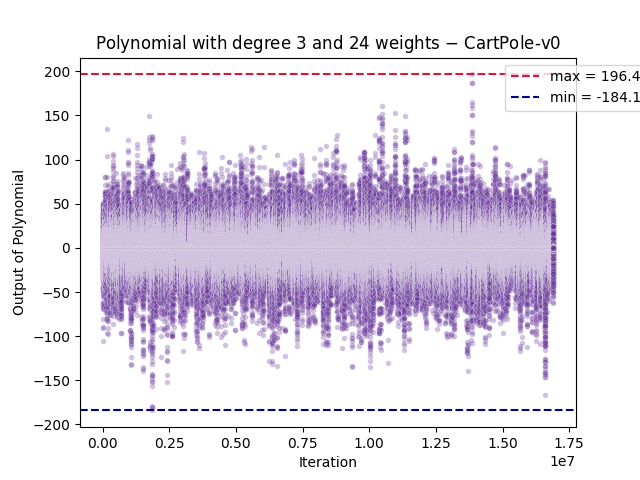
\includegraphics[width=0.6\textwidth]{PolynomialNN_degree_3_bounds}
\caption[Upper and lower bound]{
  \textbf{Upper and lower bound.}
  The figure shows each output of the polynomial functions described above. As we can see, the functions are not well bound, and there are quite a few outliers.
}
\label{fig:bounds}
\end{figure}
So, I scaled the outputs with a sigmoid function. A sigmoid function is a mathematical function that maps an arbitrary input space into an output space with a small range, for example, 0 and 1. The function has a characteristic S-shaped curve. We can interpret the output space of the sigmoid function as a probability. In this case, we search for the probability that a specific action is the reasonable one given an observation $x$. Thus, for our example with the \verb|CartPole| environment, we can interpret $sig(p_0)$ as the probability that action 0 is the correct one and $sig(p_1)$ as the probability that action 1 is the correct one. Putting this thought into a formula for $P_1$ and the \verb|CartPole| environment, we get:
\[
  P_1(x) =
  \begin{cases}1~&{\text{ if }}~sig(p_1(x)) > sig(p_0(x))~,\\0~&~\text{otherwise}~.\end{cases}
\]
For the sigmoid function, I used the logistic sigmoid function. The formula and a plot of the function are shown in Figure~\ref{fig:sigmoid}.

\begin{figure}[ht]
\centering
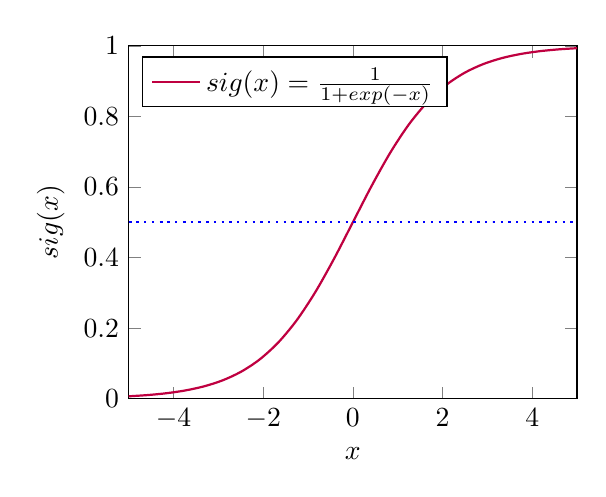
\begin{tikzpicture}
\begin{axis}[
      xmin = -5, xmax = 5,
      ymin = 0, ymax = 1,
      legend cell align = {left},
      legend pos = north west,
      width = 0.6\textwidth,
      height = 0.5\textwidth,
      xlabel = \(x\),
      ylabel = {\(sig(x)\)}
    ]
    \addplot[
        smooth,
        thick,
        purple
    ] {1 / (1 + exp(-x))};
    \addlegendentry{
    $sig(x) = \frac{1}{1 + exp(-x)}$
    }
    \addplot[
        smooth,
        thick,
        blue,
        dotted
    ] {0.5};
\end{axis}
\end{tikzpicture}
\caption[Sigmoid function]{
  \textbf{Sigmoid function.}
  The figure shows a plot of the logistic sigmoid function. The function maps an arbitrary input space into the range between 0 and 1. The output of the function can be interpreted as a probability.
}
\label{fig:sigmoid}
\end{figure}


The second model $P_2$ is constructed similarly to $P_1$, but it only consists of one polynomial instead of one for each possible action. For the \verb|CartPole| environment, this means $P_2$ consists of:
\[
  p(x) = \Sigma_{i=0}^{n} w_i^T (x_k^i)_{k \in I} \in \mathbb{R}, \ \ \ \ \ \ \ \ \ \ w_i \in \mathbb{R}^4, \ \ I = \{0, 1, 2, 3\}
\]
Analogous to $P_1$, I tested the polynomial $p(x)$ with degree 1, 2, and 3. So, $n \in \{1, 2, 3\}$. In addition, I again used the logistic sigmoid function to scale the output of the polynomial. However, the output of the $P_2$ is determined by a fixed threshold instead of comparing multiple polynomials. Putting this into a formula for the \verb|CartPole| environment, we get:
\[
  P_2(x) =
  \begin{cases}1~&{\text{ if }}~sig(p(x))>0.5~,\\0~&~\text{otherwise}~.\end{cases}
\]

\todo[inline]{Explain used environments \\ Explain neural networks architecture}


\section{Results}
\subsection{Experiment 1}

\begin{figure}[!ht]
\begin{subfigure}{\textwidth}
\begin{figrow}
\item \label{row:P1_with_bias} \raisebox{-0.5\height}{
\includegraphics[width=.3\linewidth]{experiment_1/with_bias/PolynomialNN_degree_1_scatter_score.png}
\includegraphics[width=.3\linewidth]{experiment_1/with_bias/PolynomialNN_degree_2_scatter_score.png}
\includegraphics[width=.3\linewidth]{experiment_1/with_bias/PolynomialNN_degree_3_scatter_score.png}}
\item \label{row:P1_without_bias}  \raisebox{-0.5\height}{
\includegraphics[width=.3\linewidth]{experiment_1/without_bias/PolynomialNN_degree_1_scatter_score.png}
\includegraphics[width=.3\linewidth]{experiment_1/without_bias/PolynomialNN_degree_2_scatter_score.png}
\includegraphics[width=.3\linewidth]{experiment_1/without_bias/PolynomialNN_degree_3_scatter_score.png}}
\end{figrow}
\caption{Results of $P_1$}
\label{fig:results_p1}
\end{subfigure}

\begin{subfigure}{\textwidth}
\begin{figrow}
\item \label{row:P2_with_bias} \raisebox{-0.5\height}{
\includegraphics[width=.3\linewidth]{experiment_1/with_bias/Polynomial_degree_1_scatter_score.png}
\includegraphics[width=.3\linewidth]{experiment_1/with_bias/Polynomial_degree_2_scatter_score.png}
\includegraphics[width=.3\linewidth]{experiment_1/with_bias/Polynomial_degree_3_scatter_score.png}}
\item \label{row:P2_without_bias}  \raisebox{-0.5\height}{
\includegraphics[width=.3\linewidth]{experiment_1/without_bias/Polynomial_degree_1_scatter_score.png}
\includegraphics[width=.3\linewidth]{experiment_1/without_bias/Polynomial_degree_2_scatter_score.png}
\includegraphics[width=.3\linewidth]{experiment_1/without_bias/Polynomial_degree_3_scatter_score.png}}
\end{figrow}
\caption{Results of $P_2$}
\label{fig:results_p2}
\end{subfigure}
\caption[Results of experiment 1]{
  \textbf{Results of experiment 1.}
   d
}
\label{fig:plots_reproduced}
\end{figure}



\todo[inline]{Change title of plots: , instead of with, $P_1 / P_2$ instead of Polynomial}
